\documentclass[12pt, a4paper]{article}
\setlength{\parindent}{0pt}
\usepackage[utf8]{inputenc}
\usepackage[spanish]{babel}
\usepackage{graphicx}
\usepackage{wrapfig}
\usepackage{caption}
\usepackage{subcaption}
\usepackage{ textcomp }
\usepackage{enumerate}
\usepackage{amssymb}
\usepackage{mathtools}
\usepackage{amsmath}
\usepackage{blkarray}

\begin{document} 
\section*{Trabajo Práctico Final 2019}
\subsection*{Probabilidad y Estadística}
\subsection*{Ejercicio 1}
En cada ronda de un juego, un jugador gana $\mathdollar$1, con probabilidad \textit{p}, o pierde $\mathdollar$1, con probabilidad 1-\textit{p}. El jugador comienza con $\mathdollar$\textit{k}. El juego se detiene cuando el jugador pierde todo su dinero o gana un total de $\mathdollar$ \textit{n}, donde \textit{ n \textgreater k}. Las fortunas sucesivas del jugador forman una cadena de Markov en \textbraceleft 0,1,…, n\textbraceright  con $X_{0}$ = k.
\begin{enumerate}[(a)]
	\item Simular la ruina del jugador para una inversión inicial de $\mathdollar$2, jugando un juego justo.
	\item Estimar la probabilidad de que el jugador llegue a la ruina antes de ganar $\mathdollar$5.
	\item Construir la matriz de transición para la cadena de markov asociada. Estimar la probabilidad en a) calculando potencias altas de la matriz.
	\item Comparar los resultados con la probabilidad exacta. 
\end{enumerate}
	Ayuda: ver rutina \textit{gamblesruin.R}.

\subsection*{Ejercicio 2}
En aplicaciones de seguridad informática, un \textit{honeypot}(o sistema trampa) es una herramienta dispuesta en una red o sistema informático para ser el objetivo de un posible ataque informático, y así poder detectarlo y obtener información del mismo y del atacante. Los datos del \textit{honeypot} son estudiados utilizando cadenas de markov. Se obtienen datos desde una base de datos central y se observan ataques contra cuatro puertos de computadoras - 80, 135, 139 y 445- durante un año. Los estados de la cadena de markov son los cuatro puertos y se incluye un nodo indicando que ningún puerto está siendo atacado (NA). Los datos de monitorean semanalmente y el puerto más atacado durante la semana es guardado. La matriz de transición para la cadena estimada para los ataques semanales es la siguiente:
 \[
\begin{blockarray}{cccccc}
 & 80 & 135 & 139 & 145 & NA \\
\begin{block}{c(ccccc)}
  80 & 0 & 0 & 0 & 0 & 1 \\
  135 & 0 & 8/13 & 3/13 & 1/13 & 1/13 \\
  139 & 1/16 & 3/16 & 3/8 & 1/4 & 1/8 \\
  145 & 0 & 1/11 & 4/11 & 5/11 & 1/11 \\
  NA & 0 & 1/8 & 1/2 & 1/8 & 1/4 \\
\end{block}
\end{blockarray}
 \]
La distribución inicial es \textit{a} =  (0,0,0,0,1).

\begin{enumerate}[(a)]
	\item Después de dos semanas, ¿cuáles son los puertos con más y menos probabilidad de ser atacados?
	\item Encontrar la distribución límite (si es que existe) de los puertos atacados. Justificar.
\end{enumerate}

\subsection*{Ejercicio 3}
Dans et al. (2012) estudian el comportamiento de delfines en presencia de embarcaciones turísticas en la Patagonia Argentina. Para ello postulan un modelo de cadena de Markov, con espacio de estados conformado por las 5 actividades primarias de los delfines : socializar (\textit{s}), viajar (\textit{t}), merodear (\textit{m}), alimentarse ( \textit{f}), descansar (\textit{r}), obteniendo la siguiente matriz de transición:

 \[
\begin{blockarray}{cccccc}
 & s & t & m & a & r \\
\begin{block}{c(ccccc)}
  s & 0.84 & 0.11 & 0.01 & 0.04 & 0.00 \\
  t & 0.03 & 0.80 & 0.04 & 0.10 & 0.03 \\
  m & 0.01 & 0.15 & 0.70 & 0.07 & 0.07 \\
  a & 0.03 & 0.19 & 0.02 & 0.75 & 0.01 \\
  r & 0.03 & 0.09 & 0.05 & 0.00 & 0.83 \\
\end{block}
\end{blockarray}
 \]
 
\begin{enumerate}[(a)]
	\item Clasificar los estados. 
	\item Estimar la distribución a largo plazo de la actividad de los delfines.
	\item  Simular y graficar una trayectoria de dicho proceso.
\end{enumerate}

\subsection*{Ejercicio 4}
 Simular 50 pasos de caminata aleatoria en el grafo correspondiente a la Figura 1.
 
 \begin{figure}[h]
    \centering
	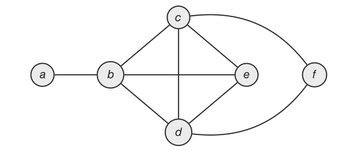
\includegraphics[scale=0.6]{img3}
	\caption{}
\end{figure}

\begin{enumerate}[(a)]
	\item Repetir la simulación 10 veces. ¿Cuántas terminaron en el vértice c?
	\item  Comparar con el resultado exacto de la probabilidad a largo plazo de visitar a c.
 \end{enumerate}
 
 \subsection*{Ejercicio 5}
Hay \textit{k} canciones en el reproductor de música de María. El reproductor está seteado en un modo \textit{shuffle}, en el cual las canciones se eligen aleatoriamente, de forma uniforme, con reemplazo. Por lo tanto, las repeticiones de canciones es posible.\\
Sea $X_n$ el número de canciones no repetidas que han sido escuchadas después de la \textit{n}-ésima reproducción.

\begin{enumerate}[(a)]
	\item Mostrar que \textbraceleft $X_n : n \in \mathbb{N} $\textbraceright  es una cadena de markov y determinar la matriz de transición.
	\item  Si María tiene cuatro canciones en su reproductor de música, encontrar la probabilidad de que todas las canciones sean escuchadas después de 6 reproducciones.
 \end{enumerate}

\subsection*{Ejercicio 6}
Se tiran 5 dados y se ponen a un lado aquellos que mostraron un 6. Los restantes se lanzan nuevamente y se repite el procedimiento, poniendo a un lado aquellos dados que muestran un 6, y así sucesivamente.
\\Sea $X_n$ el número de dados en los que salió 6 después de \textit{n} tiradas.
\begin{enumerate}[(a)]
	\item Describir la matriz de transición \textit{P} para la cadena de markov.
	\item  Encontrar la probabilidad de obtener todos 6 en tres jugadas.
	\item ¿Cómo se espera que sea $P^{100}$? Confirmar la respuesta utilizando R.
 \end{enumerate}


\subsection*{Ejercicio 7}
Considerar la caminata aleatoria en \textbraceleft 0,...,k\textbraceright, la cual se mueve a la izquierda o a la derecha con probabilidades \textit{p} y \textit{q}, respectivamente. Si el proceso está en 0, transiciona a 1 en el siguiente paso. Si el proceso está en \textit{k}, transiciona a \textit{k}-1 en el siguiente paso. Esto se llama \textit{caminata aleatoria con límites reflectantes}. Asumir que \textit{k} = 3, \textit{q} = ¼, \textit{p} = ¾ y la distribución inicial es uniforme.
\begin{enumerate}[(a)]
	\item Calcular la matriz de transición.
	\item  Encontrar P($X_7= 1 | X_0=3,X_2=2,X_4=2$) 
	\item Encontrar P($X_3=1,X_5=3$)
 \end{enumerate}

\subsection*{Ejercicio 8}
Los administradores de datos de una universidad desarrollaron un modelo markoviano para simular los índices de graduación en la institución. Los estudiantes pueden abandonar, repetir un año o pasar al año siguiente. Todos tienen un 3\% de chance de repetir el año.  Aquellos que se encuentran en primer o segundo año, tienen una chance del 6\% de abandonar. Para estudiantes de tercer y cuarto año, el índice de abandono es de 4\%. 
\begin{enumerate}[(a)]
	\item Clasificar los estados.
	\item  Establecer la matriz de transición de un paso.
	\item Determinar el número promedio de años que un estudiante que ingresa en primer año permanece en la institución antes de abandonar o recibirse.
 \end{enumerate}

\subsection*{Ejercicio 9}
El modelo Wright-Fisher describe la evolución de una población fija de \textit{k} genes. Los genes pueden ser de uno de dos tipos, llamados alelos: \textit{A} o \textit{a}. Sea $X_n$ el número de alelos A en la población en el momento \textit{n}, donde el tiempo se mide por generaciones. Bajo este modelo, el número de alelos A en el momento \textit{n}+1 se obtiene muestreando con reemplazo desde la población de genes en el momento \textit{n}. Por lo tanto, habiendo \textit{i} alelos de tipo A en el momento \textit{n}, el número de alelos A en el momento \textit{n}+1 tiene una distribución binomial con parámetros \textit{k} y \textit{p} = \textit{i/k}. Esto resulta en una cadena de markov con matriz de transición definida por:
\begin{equation}
P_{ij} = \binom{k}{j} (\dfrac{i}{k})^j (1-\dfrac{i}{k})^{k-j}, \ para \ 0\leq i, j\leq k.
\end{equation}
\begin{enumerate}[(a)]
	\item Simular este proceso para algún valor de \textit{k}.
	\item  Observar qué valor toma $P_{00}$ y $P_{kk}$.
	\item Cuando la cadena progresa, la población, en algún momento, termina con todos alelos a (estado 0) o todos alelos A (estado \textit{k}). Determinar cuál es la probabilidad de que la población evolucione al estado \textit{k}.
 \end{enumerate}

\subsection*{Ejercicio 10}
 El día de la elección, las personas participaron en un centro de votaciones de acuerdo con un proceso de Poisson. El promedio,  100 votantes llegan cada hora. 
\begin{enumerate}[(a)]
	\item Si 150 personas arribaron durante la primer hora, ¿qué probabilidad hay de que al menos 350 votantes arriban antes de las 3 horas?
	\item Simular dicho proceso y graficar una trayectoria.
	\item Considerar la variable aleatoria: tiempo entre arribos. Obtener los valores a través de simulación y graficar. Determinar qué distribución tiene el tiempo entre arribos de votantes.

 \end{enumerate}
\end{document}